\section{Benchmark}
Um die Benchmark Tests reproduzierbar zu machen gibt es hier nun zunächst eine Auflistung der Komponenten, auf denen die Tests durchgeführt wurden:
\begin{itemize}
\item NVIDIA GeForce RTX 3070
\item Intel Core i7 12700
\item 32 Gb DDR 4 RAM
\item B660 GAMING X DDR 4 Mainboard
\item Samsung SSD 850 EVO 500 Gb
\end{itemize}
In diesem Kapitel wird nun der direkte Vergleich von dem ECS und dem objektorientierten Teil angestellt. Dazu stellt Unity einige hilfreiche Tools zu Verfügung um beispielsweise die Bilder pro Sekunde, in seinem Spiel, zu messen. Auch können man dadurch gut nachvollziehen, wie lange eine Aufgabe, wie zum Beispiel die Ausführung der Update Funktionen, benötigt hat. Bei den nachfolgenden Tests wird jeweils das implementierte Spiel, welches in \hyperref[sec:factory]{Kapitel \ref*{sec:factory}} vorgestellt wurde, verwendet. Es werden immer 2000 Bilder gemessen, wobei die letzten 2000 Bilder aufgezeichnet werden, sobald ein Stahlbarren hinten in dem Kasten angekommen ist (\hyperref[fig:steel]{Abbildung \ref*{fig:steel}}). Zusätzlich werden mehrere Durchläufe gemacht. Angefangen wird mit 100 Fabriken. Diese werden in 100er Schritten erhöht bis zu 1000 Fabriken.
\subsection{Profiler}
Mit dem Profiler kann man in Unity sein Spiel aufzeichnen und Daten über eine festgelegte Anzahl von Bildern sammeln. Dazu gehören die CPU Auslastung, der Speicherverbrauch, wie viel Objekte gezeichnet werden und noch vieles mehr. Während das Spiel läuft gibt werden diese Daten live gezeigt. Zusätzlich lassen sich die Daten auch beim pausieren des Spiel abspeichern und andere Daten laden um sie zu betrachten. Dies sieht man auch in nachfolgender \hyperref[fig:profiler]{Abbildung \ref*{fig:profiler}}. 
\begin{figure}[H]
\centering
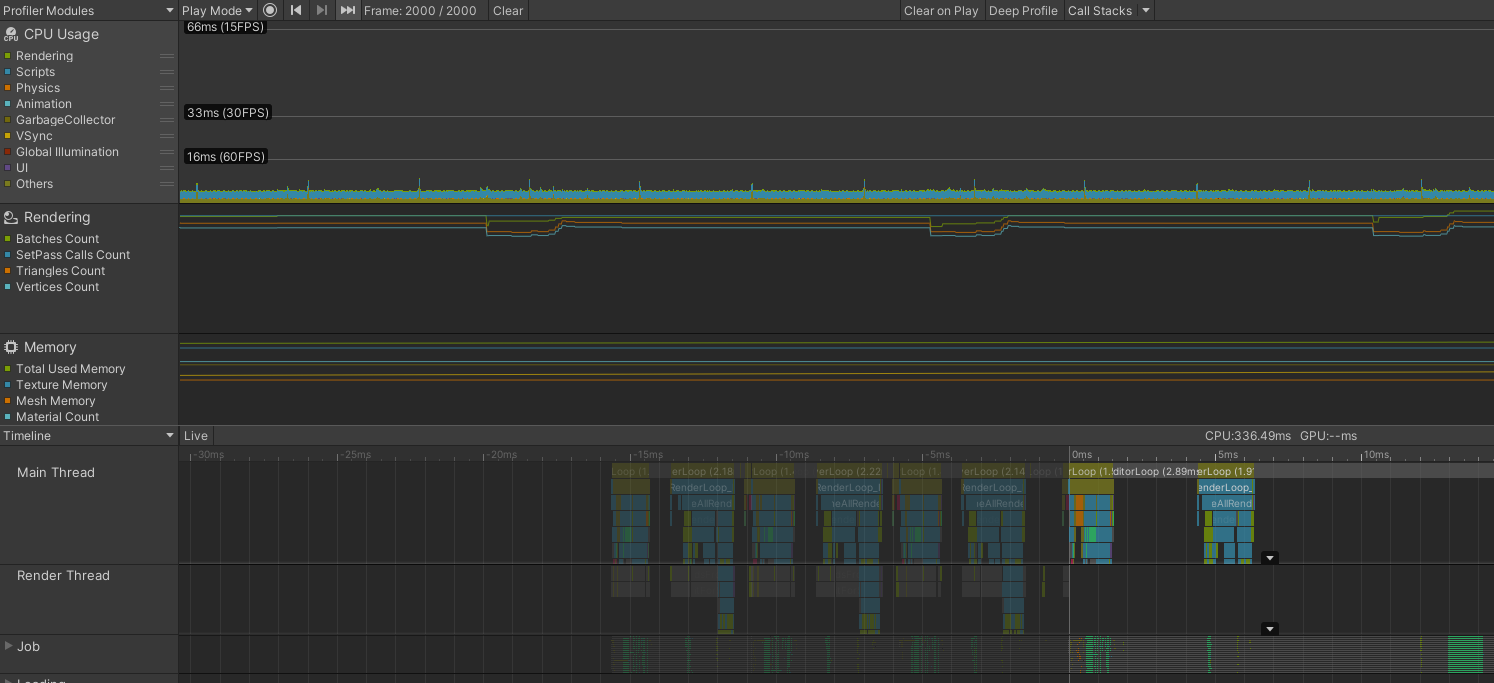
\includegraphics[scale=0.428]{Bilder/Profiler.png}
\caption{Der Profiler in dem Unity Editor. Mit ihm lässt sich die Auslastung des Spiels während dem Spielen aufzeichnen und die Daten zur weiteren Verwendung abspeichern.}
\label{fig:profiler}
\end{figure}
In dem Bild erkennt man die einzelnen Auslastungen und ihre Kategorien. Zusätzlich kann man ein bestimmtes Bild auswählen und erhält dazu weitere Details in der Timeline weiter unten. Diese aufgezeichneten Daten lassen sich dann in dem Profile Analyzer weiter analysieren.
\subsection{Profile Analyzer}
Der Profile Analyzer dient der weiteren Analyse von aufgenommenen Profilen mit dem Profiler. Zusätzlich hat man mit dem Profile Analyzer die Möglichkeit zwei Profile direkt miteinander zu vergleichen. Dies kann man in \hyperref[fig:profile_analyzer]{Abbildung \ref*{fig:profile_analyzer}} sehen.
\begin{figure}[H]
\centering
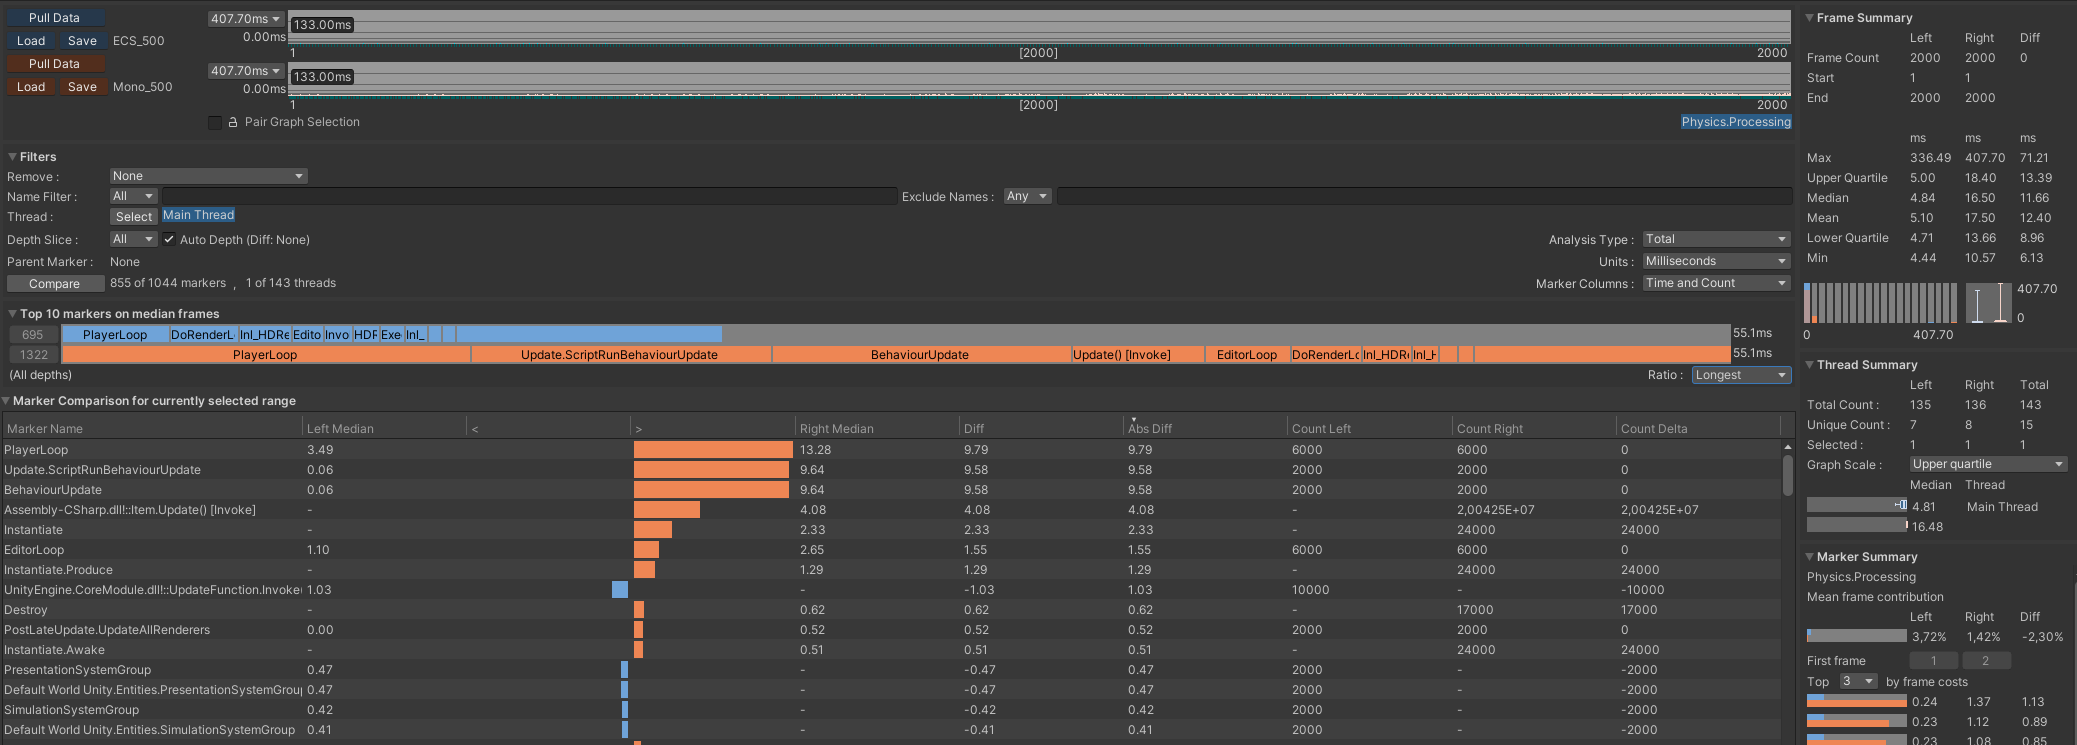
\includegraphics[scale=0.31]{Bilder/Profile Analyzer.png}
\caption{Der Profile Analyzer im Unity Editor. Es werden die Objekt- und die Datenorientierten Messdaten von dem Spiel miteinander verglichen. Das Spiel mit dem ECS ist im Bild blau dargestellt, das andere rot.}
\label{fig:profile_analyzer}
\end{figure}
Oberhalb erkennt man beide Daten die man vergleichen möchte und wie viele Bilder die beiden Daten enthalten. Hier ist erkennbar, dass einmal die Daten von dem ECS mit 500 Fabriken (blau dargestellt) und dem Objektorientierten mit 500 Fabriken (rot dargestellt) verglichen werden. Die wichtigen Teile sind hierbei die zusammenfassende Übersicht (rechts), welche eine Übersicht über alle Bilder oder Threads bietet, und den Vergleich von Kernfunktionen der Spiele, wie beispielsweise der Update Funktionen und dem erstellen, oder zerstören von Objekten. Das Problem hierbei ist jedoch, dass die Kernfunktionen von dem Objektorientierten, anders heißen als die von dem Datenorientierten und man sie somit schlecht gegenüberstellen kann. Würde man zwei Objektorientierte Spiele vergleichen, hätten beide einen PlayerLoop und man würde direkt erkennen, welcher länger gebraucht hat. Dennoch kann man die Zusammenfassung der Bilder gut Nutzen und deshalb werden diese im Folgenden ausgewertet.
\subsection{Vergleich}
\begin{figure}[H]
\centering
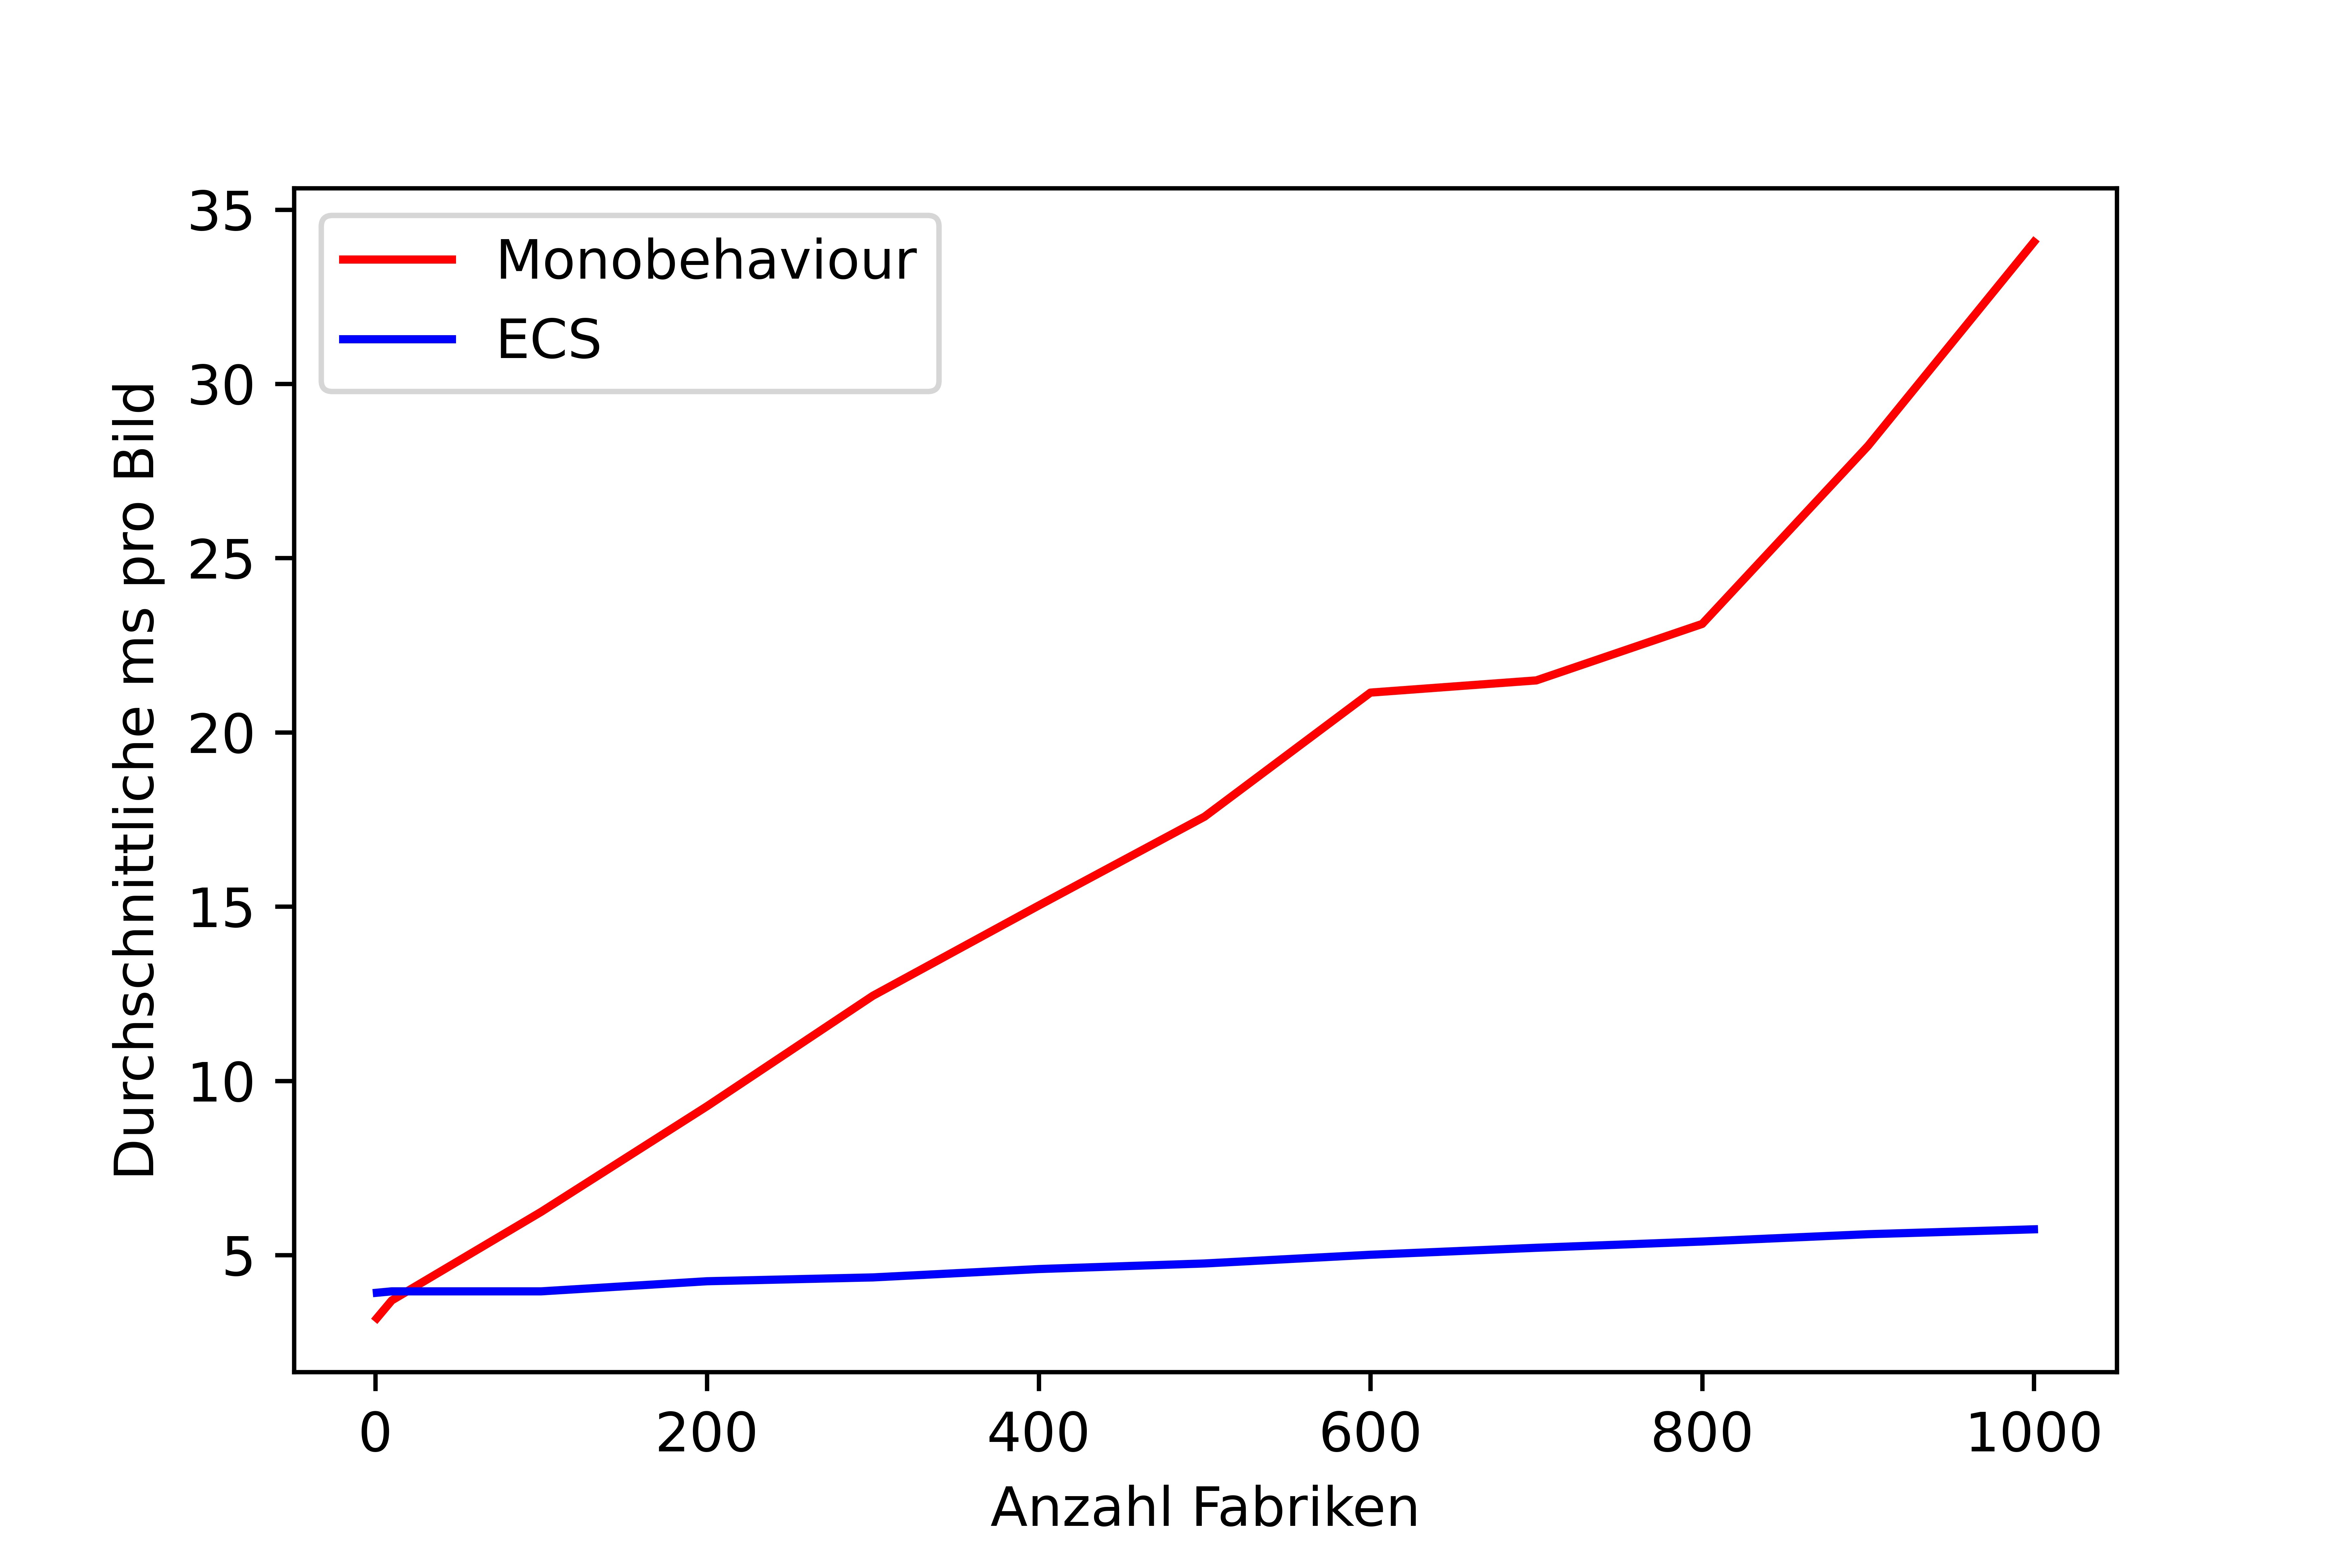
\includegraphics[scale=1]{Bilder/Benchmark.png}
\caption{Der Vergleich von Monobehaviour und dem Entity Component System. Die y-Achse zeigt die durchschnittlichen Millisekunden, die ein Bild gebraucht hat. Die x-Achse zeigt die Anzahl der Fabriken im Spiel.}
\label{fig:benchmark}
\end{figure}
In \hyperref[fig:benchmark]{Abbildung \ref*{fig:benchmark}} sieht man nun den direkten Vergleich der Laufzeiten von Monobehaviour zu dem ECS. Ganz deutlich erkennbar schneidet das Monobehaviour wesentlich schlechter ab. Das Monobehaviour braucht deutlich länger um ein Bild zu verarbeiten, gerade wenn sich die Anzahl der Fabriken erhöht. Also bestätigt das die Annahme, dass das ECS wesentlich besser darin ist große Mengen an Objekten zu verarbeiten. Auch hier steigt die durchschnittliche Zeit ein Bild zu verarbeiten, jedoch nur sehr gering. 